\section{Temperature control loop with variable dead time}
The difficulties associated with the control of deadtime processes can be investigated on this rig (shown in figure~\ref{fig:rig:heat}.
\begin{figure}
	\centering
	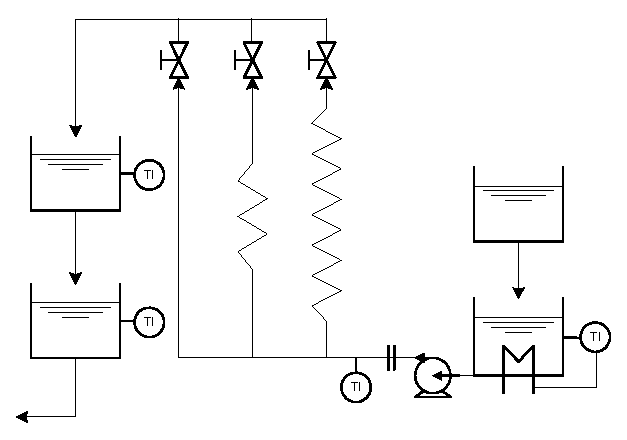
\includegraphics{Heat}
	\caption{The variable dead time temperature control rig}
	\label{fig:rig:heat}
\end{figure}
Three paths with different lengths (and different dead times) can be selected by opening and closing manual valves.  Four temperatures are measured at different points on the control loop and can be controlled by manipulating heat input from an adjustable heating element. 

\subsection{Procedures}
\subsubsection{Commissioning}
\begin{enumerate}
	\item Make a visual inspection of the equipment and ensure that no rust or obstructions are visible on the rig.  Special care should be taken to remove algal growth from the water heater.
	\item Ensure water supply is connected
	\item Ensure drain is open and unconstricted
	\item Ensure that power is supplied to the rig as well as the Thyristor
	\item Open \tagname{HV005} (Water supply valve)
	\item Ensure that water flows into the water heater
	\item Allow water level to stabilise
	\item Ensure that the float activated valve closes
	\item Follow procedure for calibrating thermocouples described in paragraph~\ref{sec:thermocouplecalibration}
\end{enumerate}

\subsubsection{Wet Startup}
This procedure is to start the rig after it has been commissioned.  There must be water in the system and the water supply must be connected with all supply valves open.
\begin{enumerate}
	\item Enable 100\% power on Thyristor
	\item Switch on mixer
	\item Ensure \tagname{HV002}, \tagname{HV003} and \tagname{HV004} are switched to the correct positions for the experiment
	\item Wait for temperature to reach setpoint temperature
	\item Switch on pump
	\item Open \tagname{HV001}
	\item Switch to automatic control on thyristor.
\end{enumerate}

\subsubsection{Shutdown}
This is the standard shutdown when the rig is still to be used in the near future.  It retains water in the rig and keeps it in readiness for a wet startup.
\begin{enumerate}
	\item Stop thyristor by pressing stop button
	\item Stop mixer
	\item Stop pump
	\item Close \tagname{HV001}
\end{enumerate}

\subsubsection{Decommissioning}
\begin{enumerate}
	\item Close \tagname{HV005}
	\item Start pump
	\item Allow tank to drain without allowing the pump to run dry
	\item Stop pump
	\item Allow water to run down from \tagname{T001} (Dead time reservoir tank)
	\item Close \tagname{HV001}
	\item Syphon off remaining water and dry tank
\end{enumerate}